\section{Introduction}
\begin{frame}{What is Deep Learning?}
    \centering
    \Large
    Deep Learning is simply \textbf{Machine Learning}...
    
    \vspace{0.5em}
    ...but powered by \textbf{Artificial Neural Networks} with many layers.
    
    \vspace{1.5em}
    \normalsize
    \begin{itemize}
        \item \textbf{"Neural":} Inspired by the human brain (neurons).
        \item \textbf{"Deep":} Refers to the number of layers (depth).
    \end{itemize}
    
    \pause
    \vspace{1em}
    \textit{But why did Deep Learning suddenly become so powerful?}
\end{frame}

% --- SLIDE 2: The Timing ---
\begin{frame}{Why Now?}
    \textit{Deep Learning isn't new. The ideas date back decades. But three things changed:}
    
    % \vspace{1em}
    \begin{columns}[c]
        \begin{column}{0.4\textwidth}
            \small
            \begin{enumerate}
                \item More \textbf{data} \\
                \small (internet, sensors, images)
                % \vspace{0.5em}
                \item Faster \textbf{compute} \\
                \small (GPUs, cloud computing)
                % \vspace{0.5em}
                \item Better \textbf{algorithms} \\
                \small (training techniques, architectures)
            \end{enumerate}
        \end{column}
        
        \begin{column}{0.5\textwidth}
            \centering
            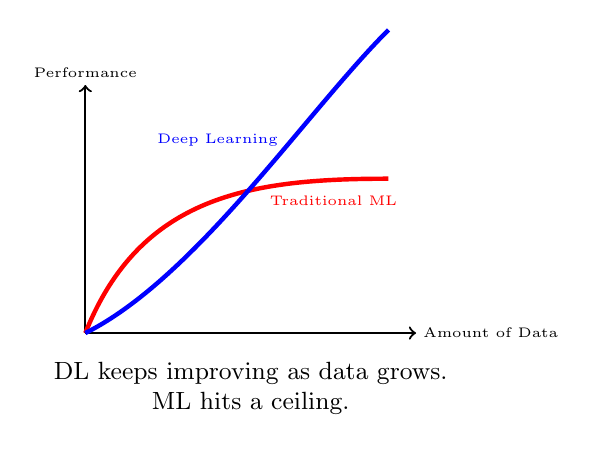
\begin{tikzpicture}[scale=0.7]
            \tiny
                \draw[->, thick] (0,0) -- (6,0) node[right] {Amount of Data};
                \draw[->, thick] (0,0) -- (0,4.5) node[above] {Performance};
                
                % ML Curve (Plateau)
                \draw[red, ultra thick] (0,0) .. controls (1,2.5) and (3,2.8) .. (5.5,2.8);
                \node[red] at (4.5, 2.4) {Traditional ML};
                
                % DL Curve (Linear Scaling)
                \draw[blue, ultra thick] (0,0) .. controls (2,1) and (4,4) .. (5.5,5.5);
                \node[blue] at (2.4, 3.5) {Deep Learning};
                
                \node[align=center, font=\small] at (3, -1) {DL keeps improving as data grows.\\ML hits a ceiling.};
            \end{tikzpicture}
        \end{column}
    \end{columns}
    
    \pause
    \vspace{0.8em}
    \centering
    \textit{But what makes Deep Learning so scalable?}
\end{frame}
% --- SLIDE 3: The Building Blocks (Comparison) ---
\begin{frame}{The Secret: Simple Building Blocks}
    \vspace{2.5em}
    \begin{columns}[c]
        % Left: Traditional ML
        \begin{column}{0.50\textwidth}
            \begin{tcolorbox}[colback=red!5, colframe=red!50, title=\textbf{Traditional ML}]
                \small
                Models are \textbf{fixed equations} designed by experts with specific assumptions about the data.
                \vspace{0.5em}
                
                \textit{Example: Linear Regression}
                $ y = w_1 x + w_0 $
                
                \vspace{0.5em}
                \textbf{Benefit:} Fast and interpretable (when assumptions hold).
                
                \vspace{0.3em}
                \textbf{Problem:} Hard to adapt when data nature is different or unknown.
            \end{tcolorbox}
        \end{column}
        
        % Right: Deep Learning
        \begin{column}{0.50\textwidth}
            \begin{tcolorbox}[colback=blue!5, colframe=blue!50, title=\textbf{Deep Learning}]
                \small
                Models are built from \textbf{simple, stackable blocks} (like LEGO).
                \vspace{0.5em}
                
                \textit{Example: Stacking layers}
                \vspace{0.5em}
                \centering
                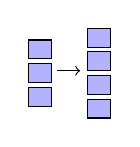
\begin{tikzpicture}[scale=0.3, baseline]
                    \foreach \y in {0,1,2} \draw[fill=blue!30] (0,\y) rectangle (1,\y+0.8);
                    \draw[->] (1.2, 1.5) -- (2.2, 1.5);
                    \foreach \y in {-0.5,0.5,1.5,2.5} \draw[fill=blue!30] (2.5,\y) rectangle (3.5,\y+0.8);
                \end{tikzpicture}
                
                \vspace{0.5em}
                \raggedright
                \textbf{Benefit:} Very flexible. Can be adapted to any data type or task.
            \end{tcolorbox}
        \end{column}
    \end{columns}

    \pause
    \vspace{1.5em}
    \centering
    \textit{So what is this magic building block?}
\end{frame}

% --- SLIDE 3B: The Neuron Reveal ---
